%% Author_tex.tex
%% V1.0
%% 2012/13/12
%% developed by Techset
%%
%% This file describes the coding for rsproca.cls

\documentclass[openacc]{rsproca_new}%%%%where rsproca is the template name
\usepackage{subcaption}
\usepackage[thinc]{esdiff} % for derivatives
\usepackage{empheq} % boxed equations

\definecolor{myboxcolor}{rgb}{0.96, 0.96, 0.96}
\newcommand*\mybox[1]{%
\colorbox{myboxcolor}{\hspace{1em}#1\hspace{1em}}}

% from empheq pkg
\definecolor{shadecolor}{rgb}{0.97, 0.97, 1.0}
\definecolor{light-blue}{rgb}{0.96, 1.0, 0.98}
\newsavebox{\mysaveboxM} % M for math
\newsavebox{\mysaveboxT} % T for text
\newcommand*\Garybox[2][Example]{%
\sbox{\mysaveboxM}{#2}%
\sbox{\mysaveboxT}{\fcolorbox{black}{light-blue}{#1}}%
\sbox{\mysaveboxM}{%
\fcolorbox{black}{shadecolor}{%
\makebox[\linewidth-10em]{\usebox{\mysaveboxM}}%
}%
}%
\usebox{\mysaveboxM}%
\makebox[0pt][r]{%
\makebox[\wd\mysaveboxM][c]{%
\raisebox{\ht\mysaveboxM-0.5\ht\mysaveboxT
+1.6\dp\mysaveboxT-0.5\fboxrule}{\usebox{\mysaveboxT}}%
}%
}%
}

%%%% *** Do not adjust lengths that control margins, column widths, etc. ***

%%%%%%%%%%% Defining Enunciations  %%%%%%%%%%%
\newtheorem{theorem}{\bf Theorem}[section]
\newtheorem{condition}{\bf Condition}[section]
\newtheorem{corollary}{\bf Corollary}[section]
%%%%%%%%%%%%%%%%%%%%%%%%%%%%%%%%%%%%%%%%%%%%%%%

%%%%% Please insert respective article type here %%%%
\titlehead{Research}

\begin{document}

%%%% Article title to be placed here
\title{Bayesian inference of the shape of an object inside of a draining tank}

\author{%%%% Author details
Gbenga Fabusola$^{1}$, 
Cory M. Simon$^{1}$
}

%%%%%%%%% Insert author address here
\address{$^{1}$School of Chemical, Biological, and Environmental Engineering. Oregon State University. Corvallis, OR, USA.
% $^{2}$Second author address\\
}

%%%% Subject entries to be placed here %%%%
\subject{applied mathematics, chemical engineering}

%%%% Keyword entries to be placed here %%%%
\keywords{inverse problems, Bayesian statistical inversion, Torricelli's law}

%%%% Insert corresponding author and its email address}
\corres{Cory M. Simon\\
\email{cory.simon@oregonstate.edu}}

%%%% Abstract text to be placed here %%%%%%%%%%%%
\begin{abstract}

\absbreak % unclear why this is needed
\end{abstract}
%%%%%%%%%%%%%%%%%%%%%%%%%%%

\rsbreak

%%%%%%%%%% Insert the texts which can accomdate on firstpage in the tag "fmtext" %%%%%

\section{Introduction}
Throughout engineering and the applied sciences, we encounter a liquid-holding tank that is draining via gravity-driven flow through a small orifice.
Mathematical models of the dynamics of the liquid level in a draining tank are useful for designing the geometry of the tank and orifice, predicting the emptying time, forecasting the outlet flow rate, controlling the liquid level via an input stream, and inferring the liquid level from the outlet flow rate \cite{d2021torricelli,seborg2016process,groetsch1993inverse,groetsch1999inverse}.

Interestingly, ancient societies (e.g. ancient Greece) exploited the empirically predictable dynamics of the water level in a draining tank to measure and display the passage of time.
Specifically, the outflow \emph{clepsydra}, Greek for ``water thief'', was an open-top container with a small hole near its bottom and graduated markings on the inside. 
Filled with water then allowed to drain, the elapsed time was indicated by the liquid level with respect to the markings on the inside. \cite{bedini1962compartmented,hwang2021historical,ritner2016oriental,hejun1987research,schomberg2018karnak,mills1982newton}
The preserved Karnak clepsydra from $\sim$1300 BC \cite{schomberg2018karnak} is an inverted truncated cone. Notably, this geometry does not provide a constant rate of decrease in the liquid level; perhaps, though, its wider top was intended to compensate for faster outflow at higher liquid levels.

%Draining tanks have been studied since ancient times, as evidenced by water clocks in ancient Egypt, Greece, India, and China.
%The water clock, or clepsydra (Greek for ''water thief''), of the outflow design consisted of an open-top container, filled with water at some reference time, with a small orifice for outflow near its bottom.

%The geometry of an ideal clepsydra would produce a constant rate of decrease in the liquid level. However, the geometry of e.g. the preserved Karnak clepsydra from $\sim$1300 BC \cite{schomberg2018karnak}, an inverted truncated cone, does not. Though, perhaps, its wider top was intended to compensate for the faster outflow when the liquid level is higher.

% Italian physicist and mathematician 
Evangelista Torricelli (1608-1647) made a fundamental observation for mathematical modeling the liquid level in a tank draining via gravity-driven flow through a small orifice: the velocity $v$ at which liquid flows out of the orifice is proportional to the square root of the height of liquid above the orifice, $\Delta h$, i.e. $v\propto \sqrt{\Delta h}$ \cite{mills1982newton}.
% TODO: check that he didn't know g!
Today, we recover Torricelli's observation from Daniel Bernoulli's (1700–1782) equation \cite{welty2020fundamentals}, a mechanical energy balance applied to the steady, plug flow of an incompressible, inviscid fluid through the orifice, with frictional forces neglected. This gives \emph{Torricelli's law}: $v=\sqrt{2 g \Delta h}$, with $g$ the acceleration due to gravity. \cite{d2021torricelli,teoman2022discharge}

Applying a mass balance and Torricelli's law to a tank draining of liquid via gravity-driven flow through a small orifice, we obtain a first-order, [generally] nonlinear differential equation governing the liquid level in the tank over time \cite{groetsch1993inverse,seborg2016process,debook}.
The geometry of the tank affects the dynamics of the liquid level through its cross-sectional area (parallel to the ground) as a function of height.
The cross-sectional area of the orifice theoretically gives the volumetric flow rate out of the tank from Torricelli's law. 
% TODO: a name for cross-sectional area parallel to the ground?
However, for the model to agree with the experimentally measured liquid level in a draining tank over time \cite{de2000pin,blasone2015discharge,wadhwa2021study,liu2008drainage}, a discharge coefficient, defined as the ratio of the observed outlet volumetric flow rate to that predicted by Torricelli's law and the area of the orifice \cite{hicks2014determining}, is introduced into the model. 
The discharge coefficient, typically around 0.6,
accounts for frictional losses across the orifice, non-uniformity of the velocity profile, and the vena contracta of the liquid jet.
The latter phenomenon of narrowing, i.e. where the cross-sectional area of the liquid jet issuing from the orifice is smaller than the area of the orifice, is due to fluid streamlines inside of the tank near the edge of the orifice with orientation not perpendicular to the area of the orifice \cite{horsch2020simple}. 
%  and (ii) depends on the rheology of the fluid and the geometry of the orifice. 
\cite{teoman2022discharge,hicks2014determining,blasone2015discharge,lienhard1984velocity,wadhwa2021study}

% Note, Torricelli's law combined with kinematic equations on a packet of fluid ejected from the orifice of the tank give the trajectory of the liquid jet, too \cite{groetsch1999inverse}.

A draining tank is an intuitive, relatable physical system to mathematically model in an undergraduate course. 
More, experiments in the classroom to collect data to validate the model of the liquid level over time are accessible and illustrate the effectiveness of mathematical models.
\cite{farmer1992physical,driver1998torricelli,brady2009siphons,rother2024modelling,paldy1963apparatus,ivanov2014testing,williams2021vessel,pavesi2019investigating,planinvsivc2011holes,saleta2005experimental,lopac2015water,powell2012carrying}
Draining tanks provide undergraduate-friendly inverse problems \cite{groetsch1993inverse,neto2012introduction,tarantola2005inverse} as well, such as inferring the shape of the tank from the observed liquid level over time \cite{groetsch1993inverse,groetsch1999inverse}. 
An inverse problem pertaining to an outflow clepsydra is: what container shape gives a constant rate of decrease in the liquid level as it drains?
(Such a clepsydra may be obtained via a solid of revolution about the vertical axis such that the radius is proportional to the quartic root of the height. \cite{mills1982newton,d2021torricelli})

In this article, we consider the following inverse problem pertaining to a tank draining of liquid
practically important:
interesting: infer a function. 


\section{Experimental setup}
In our experimental setup, we (1) fill a small, open-top, plastic tank with water, to an initial level $h_0$ [cm], then (2) at time $t=0$ [s], allow the water to drain out through a small orifice in the side of the tank, near its bottom. 
We use a liquid level strip to measure the water level in the tank over time, giving time series data $\{(t_i, h_i)\}$. The tank may or may not have a heavy, solid, stationary object inside of it, displacing water and thus affecting the dynamics of emptying. Fig.~\ref{fig:photo_of_tank} shows a photo of an experiment where the tank does not have an object inside of it.

Ultimately, we conduct a set of three experiments. The first two [repeat] experiments concern the tank without the object, for the purpose of gathering data to calibrate then test a dynamic mathematical model of the liquid level in the tank. The third experiment concerns the tank with an object inside of it, for the purpose of indirectly gathering data about then inferring the shape of that object.

\begin{figure}[h!]
\begin{center}
	% \includegraphics[width=0.3\textwidth]{../tank_geometry/photo_of_tank.png}
	\caption{\textbf{Experimental setup.} 
	The water-holding tank is shaped as inverted, right, truncated cone with a rounded rectangle base and has a small hole in its side. In our experiments, we fill the tank with water, then allow the tank to drain via gravity-driven flow out of the small hole. A liquid level strip measures the liquid level in the tank over time, giving time series data.
	}
	\label{fig:photo_of_tank}
\end{center}
\end{figure}

\paragraph{The tank geometry.} The water-holding tank is approximately an inverted, right, truncated cone with a rounded rectangle as its base. The cross-sectional area [parallel to the ground] of the tank as a function of height $h$ [cm] from its bottom base is:
\begin{equation}
	a(h) = \frac{h}{H}a_1 + \left(1-\frac{h}{H}\right) a_0,
\end{equation}
with $H$ [cm] the height of the tank and $a_0$ [cm$^2$] and $a_1$ [cm$^2$] the area of the rounded rectangle forming the bottom and top, respectively, base of the tank.
The top of the tank is open to the atmosphere. 

\paragraph{The small orifice in the side of the tank.} The tank has a small, circular hole of radius $r_o$ [cm] in its side, whose center is a small height $h_o$ [cm] from the bottom base.
Thus, when the liquid level in the tank is larger than $h_o$, water flows out of this small orifice.
(When drilling the hole, we held the drill bit parallel to the floor.) 

\paragraph{The object [possibly] inside the tank.} We may place a heavy (denser than water), solid object inside the tank. Because the object is solid, it displaces water while in the tank. Because this object is heavy, it remains at rest, at the bottom of the tank, throughout the experiment. Let $a^\prime(h)$ be the cross-sectional [parallel to the floor] area of this object as a function of height $h$.

\paragraph{The liquid level sensor.} We place a liquid level strip vertically inside the tank to measure the water level in the tank over time. The liquid level sensor communicates with an Arduino microcontroller, allowing us to automatically collect the time series data and write it to a file. The liquid level strip functions by virtue of water coming into contact with it and changing the electrical resistance. 
% TODO look at manual
We constructed a calibration curve with a resolution of 1 cm to map the reading of the level sensor [V] to the liquid level in the tank [cm]. 
% what are the units of the reading of liquid level sensor

\section{The forward and measurement models}
The \emph{forward model} provides a prediction of the liquid level $h(t)$ [m] in our draining tank over time $t$ [s], \emph{given} the shape of the tank $a(h)$, the shape of the object inside our tank $a^\prime(h)$, the radius of the circular orifice $r_o$, the height $h_o$ of the orifice, the discharge coefficient $c$, and the initial liquid level $h_0$. 
Coupled with a probabilistic \emph{measurement model} describing the noise contaminating a measurement $(t_i, h_i)$ by our liquid level sensor, the forward model allows us to compute the \emph{likelihood function}. The likelihood function specifies the probability of observing a time series data set $\{(t_i, h_i)\}$ from our experiment conditioned upon proposed functions/values for $a(h)$, $a^\prime(h)$, $r_o$, $h_o$, $c$, and $h_0$. Thus, when these functions/values are uncertain/unknown, the likelihood function scores the support that the time series data $\{(t_i, h_i)\}$ lend for each possibility.

Now, suppose we fill our tank to an initial liquid height $h_0 \leq H$ [m], then at time $t=0$ [s] allow it drain through the orifice without further input of liquid. Fundamentally, the outflow is driven by gravity exerting a force on the water above the orifice, which creates a hydrostatic pressure in the water inside the tank at the entrance of the orifice. 
We wish to model the height of liquid in the tank as a function of time, $h=h(t)$, with $t$ [s] time. 

We assume the drainage rate is sufficiently slow to keep the water at the top of the tank flat. We treat the water as incompressible (hence, constant density, $\rho$ [g/cm$^3$]) and inviscid. We do not attempt to explicitly model the flow streamlines inside the tank (as in Refs.~\cite{mathew2014numerical,sakri2017numerical}). 

\paragraph{Torricelli's law.}
Given the height of water in the tank is $h(t)$ [cm] at some time $t$, we model the velocity $v$ [cm/s] of the jet of water flowing out of the orifice with Torricelli's law \cite{d2021torricelli}:
\begin{equation}
	v\left(h(t) \right)=  \sqrt{2 g(h(t)-h_o)}, \label{eq:Torricelli}
\end{equation} where $g$ [cm/s$^2$] is the acceleration due to gravity. Torricelli's law follows from Bernoulli's equation \cite{welty2020fundamentals}, a mechanical energy balance on the flow through the orifice, treating (i) the flow as steady, plug, and frictional-lossless and (ii) the water as inviscid and incompressible.
An intuitive explanation of Torricelli's law is as follows. 
Conceptually, over a small time interval during draining, a small slice of liquid at the very top of the tank is removed and, concomitantly, an equivalent mass $m$ [g] of liquid is ejected from the orifice. Gravitational potential energy is converted to kinetic energy. 
Torricelli's law equates the loss in gravitational potential energy of the system, $m g(h-h_o)$, with the kinetic energy gained, $m v^2/2$ \cite{groetsch1993inverse,driver1998torricelli,williams2021vessel}. 

\paragraph{Volumetric flow rate out of the tank.} Given the height of water in the tank is $h(t)$ [cm] at some time $t$, we apply Torricelli's law in eqn.~\ref{eq:Torricelli} model the volumetric flow rate of water out of the tank as:
\begin{equation}
	c \pi r_o^2 \sqrt{2 g(h(t)-h_o)}, \label{eq:outletflow}
\end{equation}
with $c\in(0,1)$ the [dimensionless] discharge coefficient to account for the vena contracta in the liquid jet, non-plug flow through the orifice, and frictional losses as the water flows through the orifice. 
Note, $c=1$ assumes the area of the liquid jet is equal to that of the (circular) orifice, $\pi r_o^2$, plug flow, and no frictional losses.
Generally, the discharge coefficient depends on the rheology of the fluid, the geometry of the orifice, and, for laminar as opposed to turbulent flow, the Reynolds number of the flow \cite{teoman2022discharge}. 
\cite{horsch2020simple,teoman2022discharge,hicks2014determining,blasone2015discharge,lienhard1984velocity,wadhwa2021study}

\paragraph{Volume of water in the tank.} Given the height of water in the tank is $h(t)$ [cm] at some time $t$, the volume $V$ of water inside the tank follows from the method of cross-sections in calculus \cite{debook}:
\begin{equation}
	V(h(t))=\int_0^{h(t)} \left( a(y) - a^\prime(y) \right) dy, \label{eq:volume}
\end{equation}
where $a(y)-a^\prime(y)$ is the cross-section of water in the tank when the liquid level is $h=y$. Subtraction of the area of the object $a^\prime(y)$ accounts for the displacement of water by the object inside the tank. 

\paragraph{Mass balance.} Application of the law of conservation of mass to the draining tank (the control volume) at time $t \geq 0$ equates the rate of deaccumulation of water in the tank [g/s] with the outflow rate [g/s] using expression \ref{eq:outletflow}:
\begin{equation}
	\overbrace{\diff{}{t} \Bigl( \rho V(h(t)) \Bigr )}^{\text{rate of accumulation}}= - \overbrace{\rho c \pi r_o^2 \sqrt{2 g(h(t)-h_o)}}^{\text{outflow rate}}
\end{equation}
Taking the derivative of $V(h(t))$ in eqn.~\ref{eq:volume} and using the chain rule \cite{debook} gives our forward model for $h(t)$:
%\begin{empheq}[box=\mybox]{align}
\begin{empheq}[box={\Garybox[forward model]}]{align}
& \left(a(h)-a^\prime(h)\right) \diff{h}{t}= -c \pi r_o^2 \sqrt{2g (h(t)-h_o)}, \,\,\, t \geq 0 \label{eq:forward_model} \\
& h(0)=h_0,
\end{empheq}

a [generally] nonlinear, first-order differential equation in $h(t)$ subject to an initial condition.
Given the tank and object geometry through $a(h)$ and $a^\prime(h)$, the discharge coefficient $c$, the orifice radius and height $r_o$ and $h_o$, and initial height $h_0$, we may numerically solve the ODE in eqn.~\ref{eq:forward_model} (using e.g. \texttt{DifferentialEquations.jl} \cite{rackauckas2017differentialequations}) to predict the dynamics of the liquid level $h(t)$. 
This is a \emph{forward} model because it makes predictions forward in time, using the known causal factors that influence the dynamics of $h(t)$. 

\section{Results}
\subsection{Bayesian calibration of the dynamic model of the liquid level}

\subsection{Bayesian inference of the shape of an object inside the tank}

\section{Conclusions and Discussion}

\section{Methods}

\subsection{Details of the forward model}
Here, we build the forward model governing the height of liquid in the tank $h(t)$ [m] as a function of time $t$ [s].

\paragraph{The water in the tank.} We approximate the water in the tank as incompressible, hence having constant density $\rho$ [g/cm$^3$]. 
We assume the outflow is sufficiently slow so as to keep the water at the top of the tank as flat.
We do not explicitly model the flow lines of water internal to the tank.
% TODO flow lines? ionno.

Note, in our modeling below, we will neglect the small volume of liquid displaced by the level strip.






\paragraph{Volume of liquid in the tank.}


\paragraph{Mass balance.}
\section{The forward model}

Note: surface tension stops flow before $h=h_o$ reached.




\paragraph{Dynamic model of the liquid height in the tank.} Now, suppose we fill the tank to an initial liquid height $h_0 \leq H$ [m] at time $t=0$ [s] then allow it drain through the orifice without further input of liquid. We wish to model the height of liquid in the tank as a function of time, $h=h(t)$, with $t$ [s] time. 
A mass balance on water for $t\geq 0$, with the tank serving as the control volume, implies a volume balance if we treat the water as incompressible (constant $\rho$). The volume of liquid in the tank at time $t$ is:
\begin{equation}
	\left ( \int_0^{h(t)} \rho(y) [a(y) - a^\prime(y)]dy \right) 
\end{equation}



This gives:
\begin{equation}
\overbrace{(3e - 4f)}^{\text{text 4}}
	\frac{d}{dt} \left ( \int_0^{h(t)} \rho(y) [a(y) - a^\prime(y)]dy \right) = - \rho c \pi r_o^2 \sqrt{2 g(h(t)-h_o)},
\end{equation}
with $c\in(0,1)$ the discharge coefficient \cite{lienhard1984velocity,hicks2014determining,wadhwa2021study,teoman2022discharge} to account for frictional losses in the flow through the orifice, the vena contracta of the liquid jet out of the tank, and the non-uniform flow profile through the orifice. The term on the right is the mass flow rate of water out of the tank, and $V(t)$ [cm$^3$] is the volume of water in the tank at time $t$. 
Since the flow rate of liquid out of the tank is small, we can treat the top of the liquid as flat and relate $V(t)$ to the height of the liquid as: 
\begin{equation}
	V(t)=\int_0^{h(t)} [a(y) - a^\prime(y)]dy,
\end{equation}
bringing the geometry of the tank and the object inside of it into play. Finally, treating the water as incompressible (constant $\rho$) gives a nonlinear, first-order differential equation for $h(t)$ subject to an initial condition:

\begin{align}
& [a(h)-a^\prime(h)]\frac{dh}{dt}= -c \pi r_o^2 \sqrt{2g (h(t)-h_o)}, \,\,\, t \geq 0 \\
& h(0)=h_0.
\end{align}


\section{Results}

\begin{figure}[h!]
    \centering
        \begin{subfigure}[b]{0.3\textwidth}
    	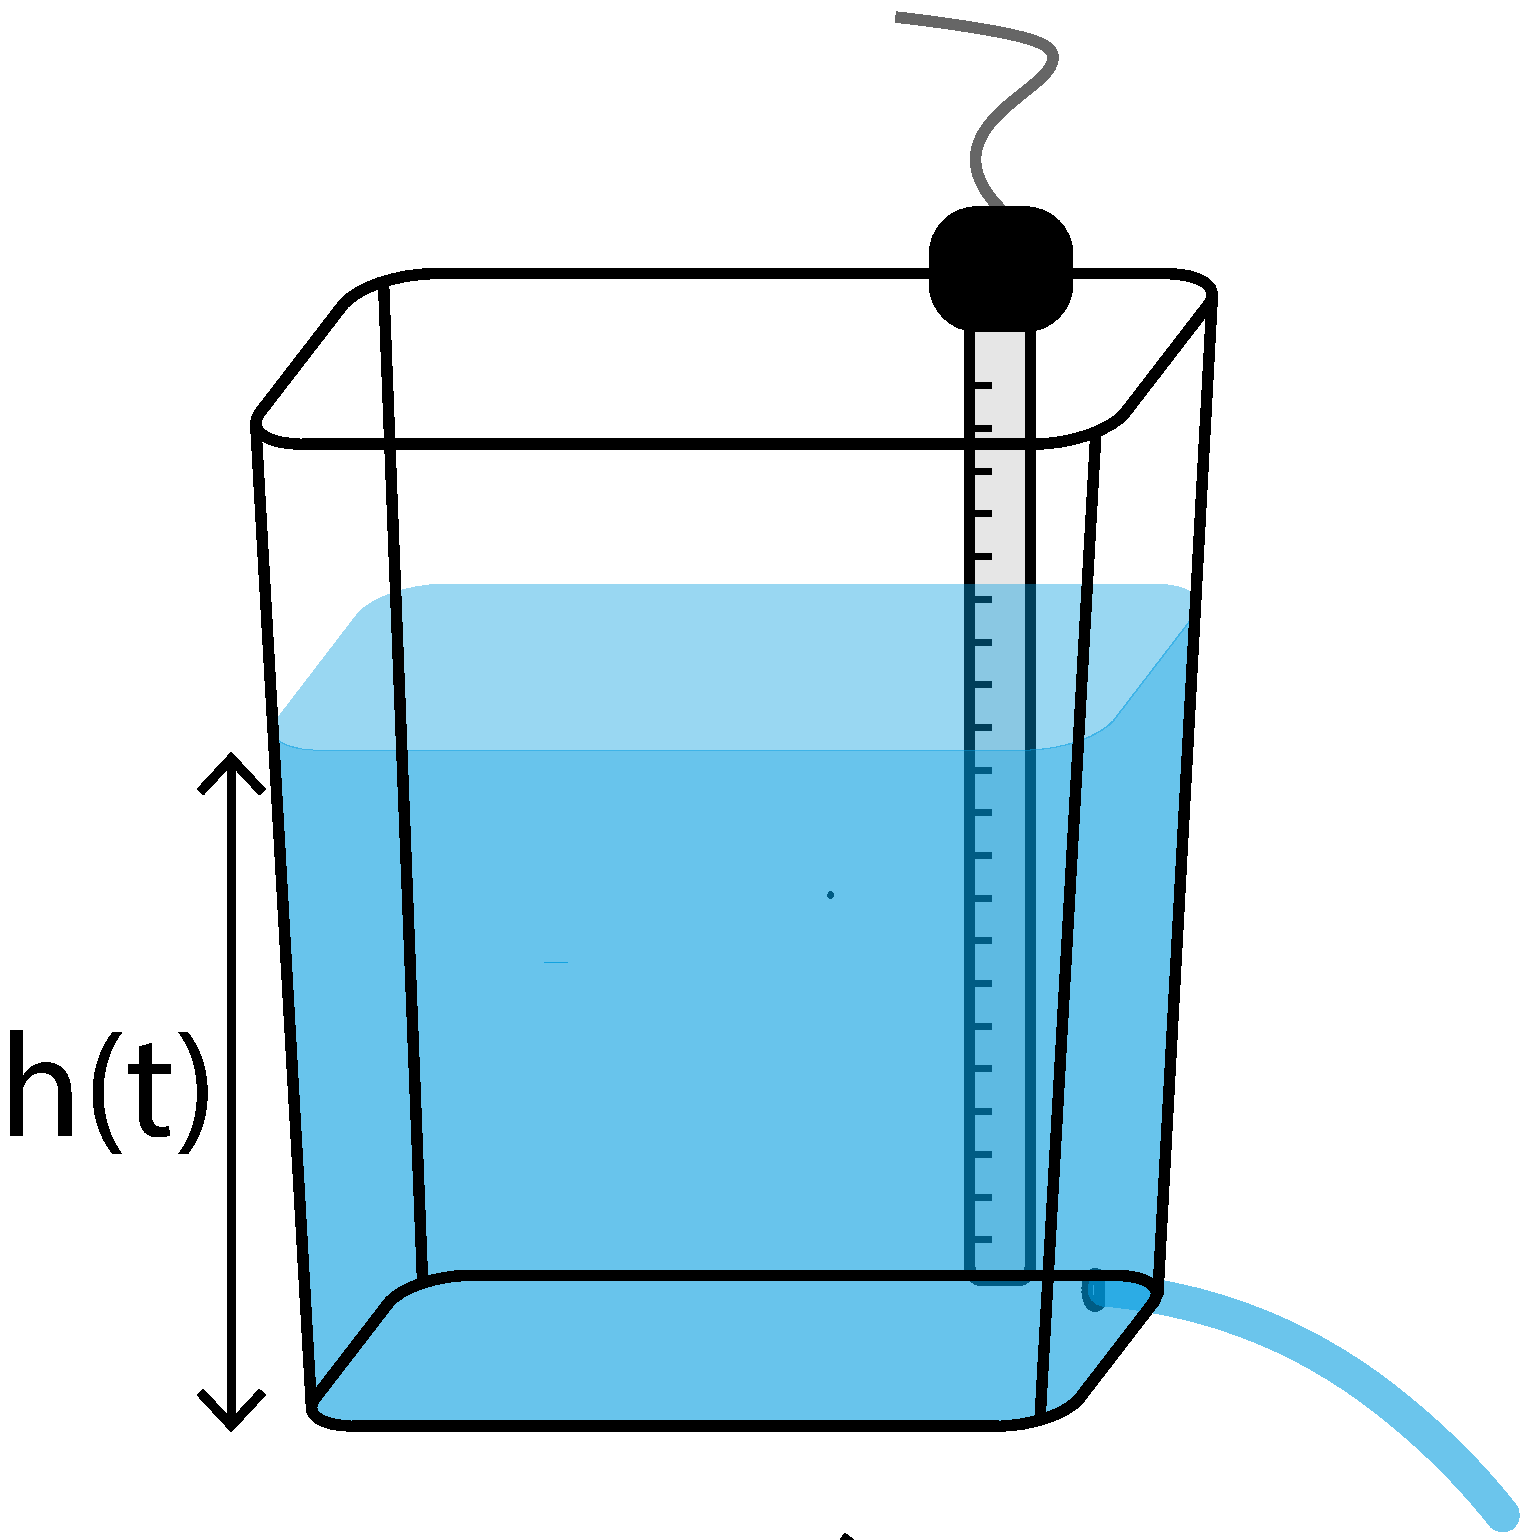
\includegraphics[width=\textwidth]{../tank_geometry/naked_tank.pdf}
	\caption{Experimental setup} \label{fig:naked_tank}
    \end{subfigure}
    
     \begin{subfigure}[b]{0.49\textwidth}
    	\includegraphics[width=\textwidth]{../prior_train.pdf}
	\caption{Prior dist'n of $h(t)$} \label{fig:prior_train}
    \end{subfigure}
     \begin{subfigure}[b]{0.49\textwidth}
    	\includegraphics[width=\textwidth]{../posterior_train.pdf}
	\caption{Data $\{(t_i, h_i)\}$ and posterior dist'n of $h(t)$} \label{fig:posterior_train}
    \end{subfigure}
    
     \begin{subfigure}[b]{0.49\textwidth}
    	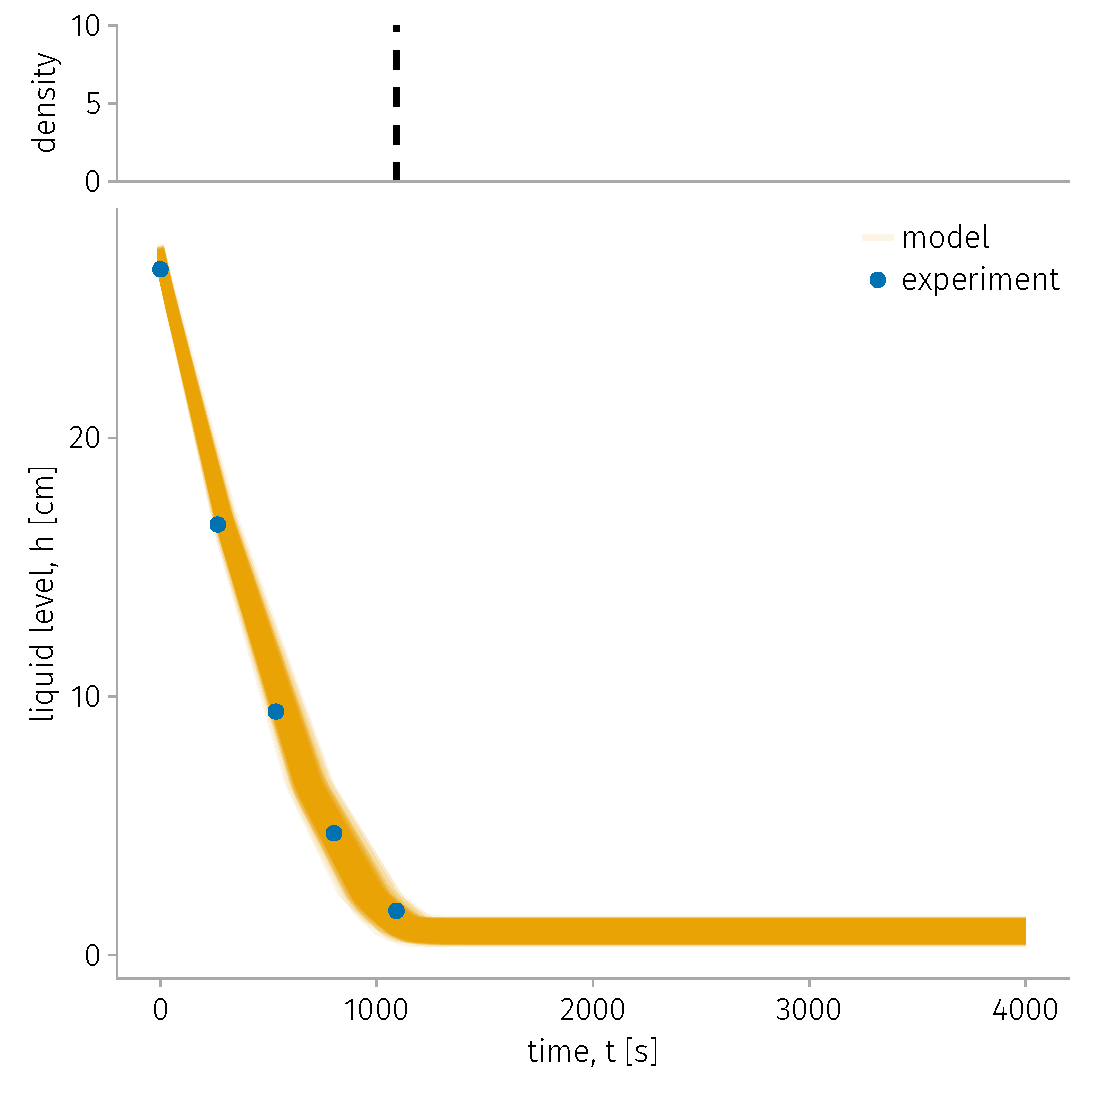
\includegraphics[width=\textwidth]{../test.pdf}
	\caption{Test} \label{fig:test}
    \end{subfigure}
    \caption{
      \textbf{Model calibration.}
      }
\end{figure}

\begin{figure}[h!]
    \centering
        \begin{subfigure}[b]{0.3\textwidth}
    	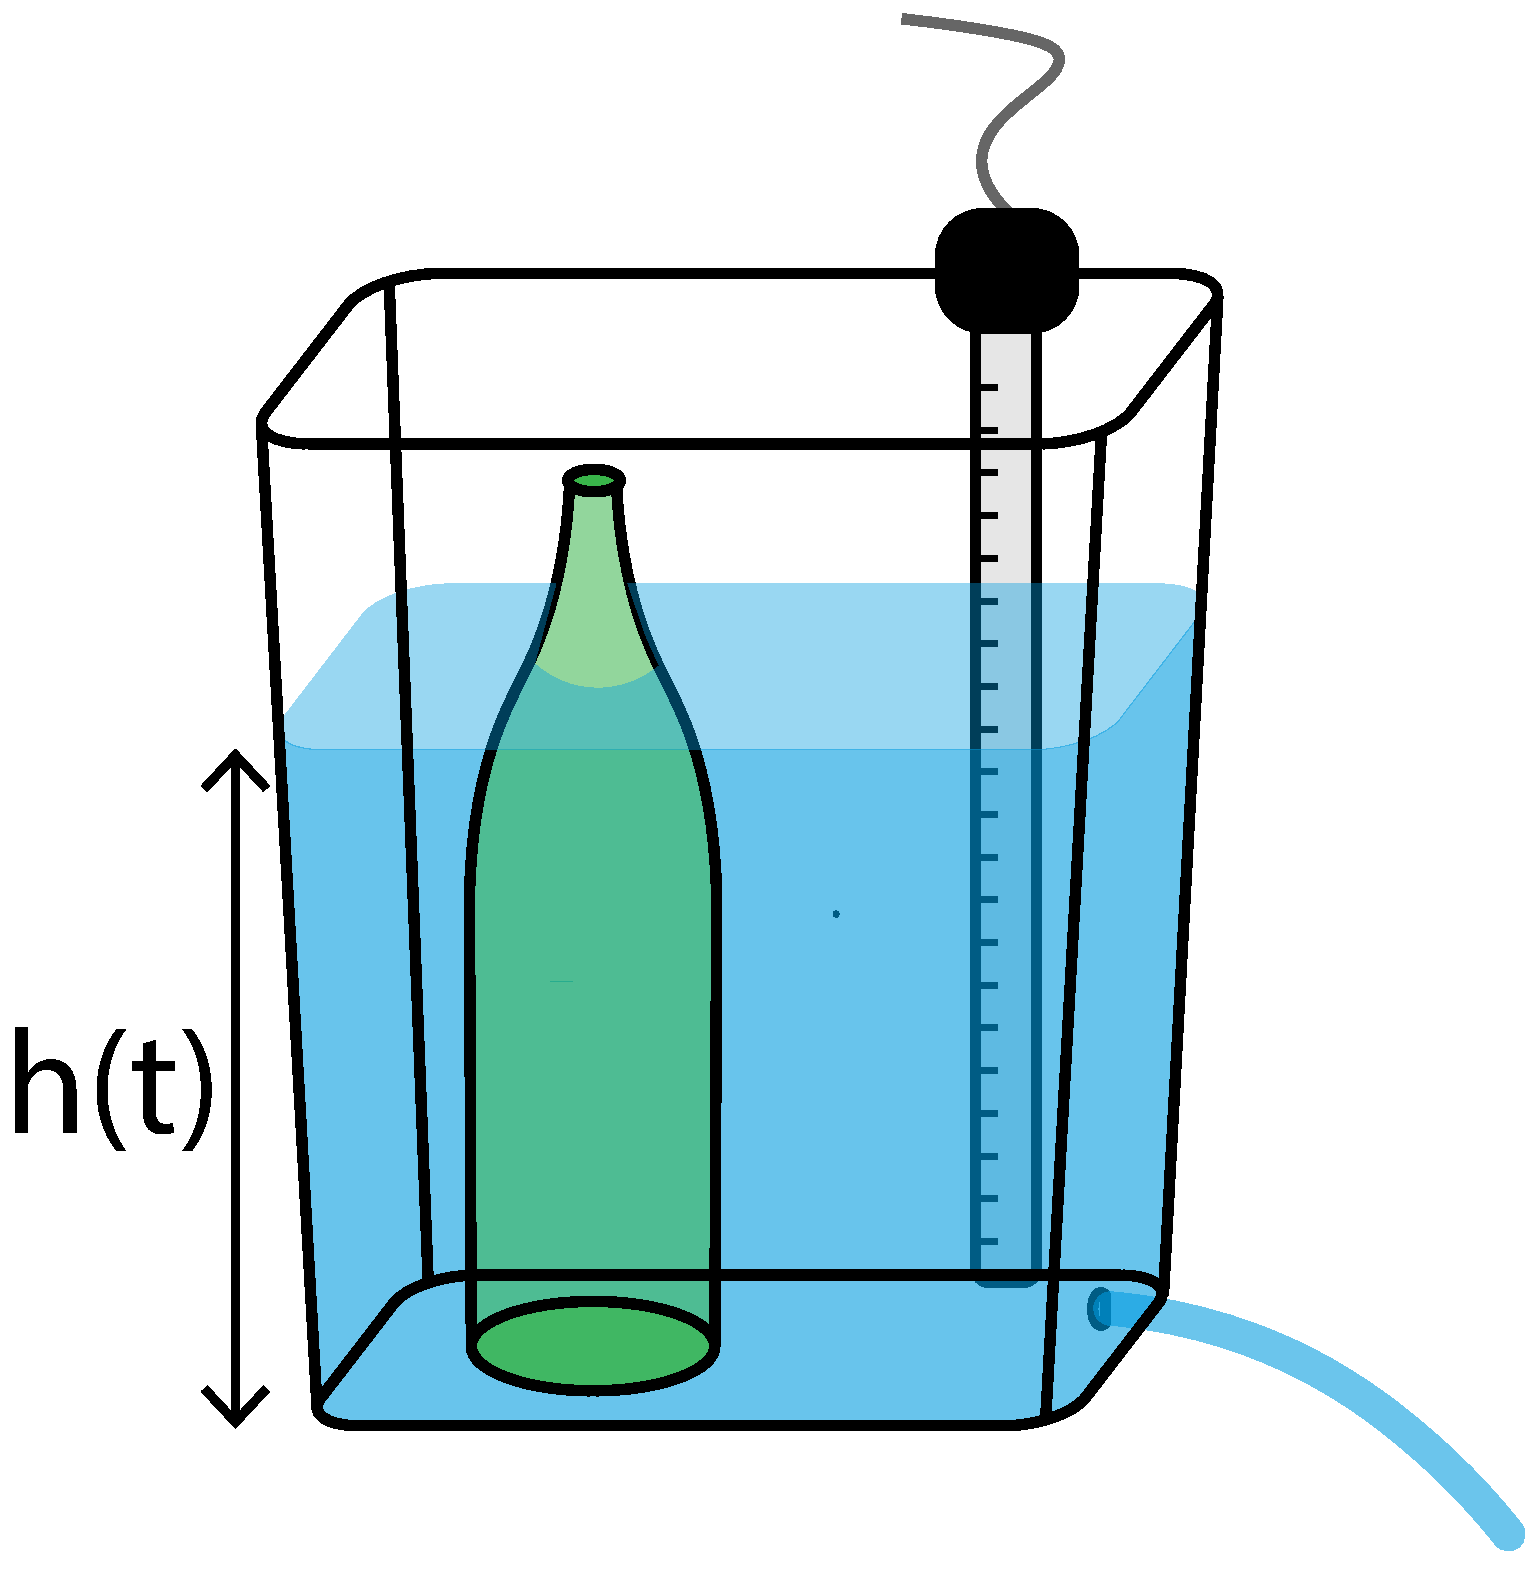
\includegraphics[width=\textwidth]{../tank_geometry/tank_w_bottle.pdf}
	\caption{Experimental setup} \label{fig:tank_w_bottle}
    \end{subfigure}
     \begin{subfigure}[b]{0.49\textwidth}
    	\includegraphics[width=\textwidth]{../posterior_object.pdf}
	\caption{Data $\{(t_i, h_i)\}$ and posterior dist'n of $h(t)$} \label{fig:posterior_object}
    \end{subfigure}
    
     \begin{subfigure}[b]{0.49\textwidth}
    	\includegraphics[width=\textwidth]{../prior_area.pdf}
	\caption{Prior dist'n of $a^\prime(h)$} \label{fig:prior_area.pdf}
    \end{subfigure}
       \begin{subfigure}[b]{0.49\textwidth}
    	\includegraphics[width=\textwidth]{../posterior_area.pdf}
	\caption{Posterior dist'n of $a^\prime(h)$} \label{fig:posterior_area.pdf}
    \end{subfigure}
    
  
    \caption{
      \textbf{Inferring the shape of the object in the tank.}
      }
\end{figure}

\section{Discussion}

Rocks inside tank. infer type of rock, coupled with packing. Popcorn polymer.

Surface tension dominates keeping the liquid from exiting. Then Torricelli's law not valid. Liquid stops emptyhing slightly above the hole. 

Mariotte's bottle \cite{kirevs2006mariotte}

\enlargethispage{20pt}

\ack{GF acknowledges ARMI for funding.}


%%%%%%%%%% Insert bibliography here %%%%%%%%%%%%%%

\vskip2pc


\bibliographystyle{RS} %%%% .BST file

\bibliography{refs} %%%%% .Bib file

\end{document}
